\documentclass[tikz]{standalone}

\usetikzlibrary{positioning,automata,calc}

\begin{document}

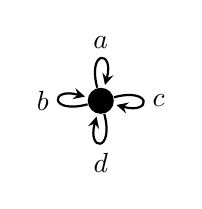
\begin{tikzpicture}[>=stealth]

\node [fill=black,black,circle] at (0,0) (s0) {};

\path[-,thick] (s0) edge [loop above] node {$a$} ();
\path[-,thick] (s0) edge [loop left]  node {$b$} ();
\path[-,thick] (s0) edge [loop right] node {$c$} ();
\path[-,thick] (s0) edge [loop below] node {$d$} ();

\end{tikzpicture}


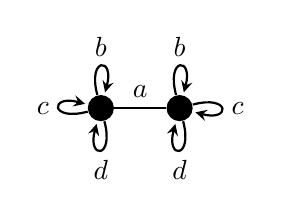
\begin{tikzpicture}[>=stealth]

\node [fill=black,black,circle] at (0,0) (s0) {};
\node [fill=black,black,circle] at (1,0) (s1) {};

\draw [thick] (s0) to node [above] {$a$} (s1);

\draw[-,thick] (s0) edge [loop above] node {$b$} ();
\path[-,thick] (s0) edge [loop left]  node {$c$} ();
\path[-,thick] (s0) edge [loop below] node {$d$} ();

\path[-,thick] (s1) edge [loop above] node {$b$} ();
\path[-,thick] (s1) edge [loop right] node {$c$} ();
\path[-,thick] (s1) edge [loop below] node {$d$} ();

\end{tikzpicture}


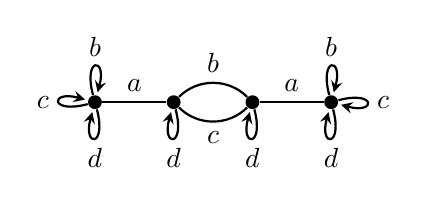
\begin{tikzpicture}[>=stealth]

\foreach \x in {0,...,3} {
	\node [fill=black,black,circle,,inner sep=0pt,minimum size=.5em] at (\x,0) (s\x) {};
	%	\path[thick] (s\x) edge [loop below] node {$d$} ();
}

\foreach \x in {0,2} {
	\pgfmathtruncatemacro{\j}{\x + 1};
	\draw [thick] (s\x) to node [above] {$a$} (s\j);
}


%\foreach \x in {1,3} {
%	\pgfmathtruncatemacro{\j}{\x + 1};
%	\draw [thick] (s\x) to [bend left] node [above] {$b$} (s\j);
%	\draw [thick] (s\x) to [bend right] node [below] {$c$} (s\j);
%}

%%%%%%%%%%%%%%%%%%%%%%%%%%%%%%%%%%%%%%%%%%%%%%%%%%%%%%%%%%%%%%%%

\draw [thick] (s1) to [bend left=45]  node [above] {$b$} (s2);
\draw [thick] (s1) to [bend right=45] node [below] {$c$} (s2);
\path[thick] (s1) edge [loop below] node {$d$} ();
\path[thick] (s2) edge [loop below] node {$d$} ();
%
%\draw [thick] (s3) to [bend left=45]  node [above] {$b$} (s4);
%\draw [thick] (s3) to [bend right=45] node [below] {$d$} (s4);
%\path[thick] (s3) edge [loop below] node {$c$} ();
%\path[thick] (s4) edge [loop below] node {$c$} ();
%
%\draw [thick] (s5) to [bend left=45]  node [above] {$c$} (s6);
%\draw [thick] (s5) to [bend right=45] node [below] {$d$} (s6);
%\path[thick] (s5) edge [loop below] node {$d$} ();
%\path[thick] (s6) edge [loop below] node {$d$} ();
%
%
\path[thick] (s0) edge [loop below] node {$d$} ();
\path[thick] (s3) edge [loop below] node {$d$} ();

%%%%%%%%%%%%%%%%%%%%%%%%%%%%%%%%%%%%%%%%%%%%%%%%%%%%%%%%%%%%%%%%


\path[-,thick] (s0) edge [loop above] node {$b$} ();
\path[-,thick] (s0) edge [loop left]  node {$c$} ();

\path[-,thick] (s3) edge [loop above] node {$b$} ();
\path[-,thick] (s3) edge [loop right] node {$c$} ();

%\node () at ($(s5)!0.5!(s6)$) {$\cdots$};

\end{tikzpicture}



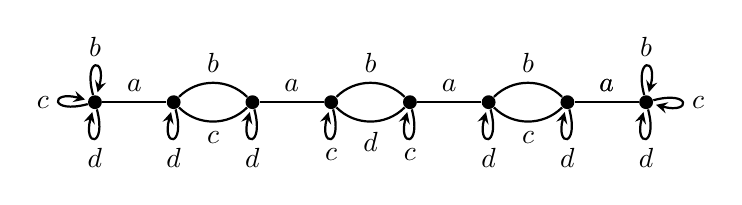
\begin{tikzpicture}[>=stealth]

\foreach \x in {0,...,7} {
	\node [fill=black,black,circle,,inner sep=0pt,minimum size=.5em] at (\x,0) (s\x) {};
%	\path[thick] (s\x) edge [loop below] node {$d$} ();
}

\foreach \x in {0,2,4,6,6} {
	\pgfmathtruncatemacro{\j}{\x + 1};
	\draw [thick] (s\x) to node [above] {$a$} (s\j);
}


%\foreach \x in {1,3} {
%	\pgfmathtruncatemacro{\j}{\x + 1};
%	\draw [thick] (s\x) to [bend left] node [above] {$b$} (s\j);
%	\draw [thick] (s\x) to [bend right] node [below] {$c$} (s\j);
%}

%%%%%%%%%%%%%%%%%%%%%%%%%%%%%%%%%%%%%%%%%%%%%%%%%%%%%%%%%%%%%%%%

\draw [thick] (s1) to [bend left=45]  node [above] {$b$} (s2);
\draw [thick] (s1) to [bend right=45] node [below] {$c$} (s2);
\path[thick] (s1) edge [loop below] node {$d$} ();
\path[thick] (s2) edge [loop below] node {$d$} ();

\draw [thick] (s3) to [bend left=45]  node [above] {$b$} (s4);
\draw [thick] (s3) to [bend right=45] node [below] {$d$} (s4);
\path[thick] (s3) edge [loop below] node {$c$} ();
\path[thick] (s4) edge [loop below] node {$c$} ();

\draw [thick] (s5) to [bend left=45]  node [above] {$b$} (s6);
\draw [thick] (s5) to [bend right=45] node [below] {$c$} (s6);
\path[thick] (s5) edge [loop below] node {$d$} ();
\path[thick] (s6) edge [loop below] node {$d$} ();


\path[thick] (s7) edge [loop below] node {$d$} ();
\path[thick] (s0) edge [loop below] node {$d$} ();

%%%%%%%%%%%%%%%%%%%%%%%%%%%%%%%%%%%%%%%%%%%%%%%%%%%%%%%%%%%%%%%%


\path[-,thick] (s0) edge [loop above] node {$b$} ();
\path[-,thick] (s0) edge [loop left]  node {$c$} ();

\path[-,thick] (s7) edge [loop above] node {$b$} ();
\path[-,thick] (s7) edge [loop right] node {$c$} ();

%\node () at ($(s5)!0.5!(s6)$) {$\cdots$};

\end{tikzpicture}




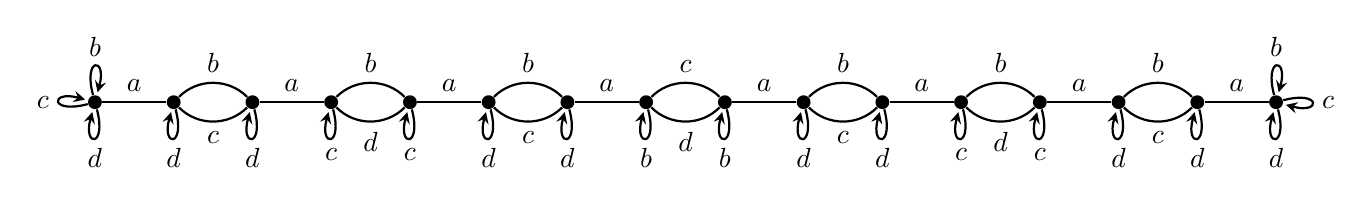
\begin{tikzpicture}[>=stealth]

\foreach \x in {0,...,15} {
	\node [fill=black,black,circle,,inner sep=0pt,minimum size=.5em] at (\x,0) (s\x) {};
	%	\path[thick] (s\x) edge [loop below] node {$d$} ();
}

\foreach \x in {0,2,4,6,8,10,12,14} {
	\pgfmathtruncatemacro{\j}{\x + 1};
	\draw [thick] (s\x) to node [above] {$a$} (s\j);
}


%\foreach \x in {1,3} {
%	\pgfmathtruncatemacro{\j}{\x + 1};
%	\draw [thick] (s\x) to [bend left] node [above] {$b$} (s\j);
%	\draw [thick] (s\x) to [bend right] node [below] {$c$} (s\j);
%}

%%%%%%%%%%%%%%%%%%%%%%%%%%%%%%%%%%%%%%%%%%%%%%%%%%%%%%%%%%%%%%%%

\draw [thick] (s1) to [bend left=45]  node [above] {$b$} (s2);
\draw [thick] (s1) to [bend right=45] node [below] {$c$} (s2);
\path[thick] (s1) edge [loop below] node {$d$} ();
\path[thick] (s2) edge [loop below] node {$d$} ();

\draw [thick] (s3) to [bend left=45]  node [above] {$b$} (s4);
\draw [thick] (s3) to [bend right=45] node [below] {$d$} (s4);
\path[thick] (s3) edge [loop below] node {$c$} ();
\path[thick] (s4) edge [loop below] node {$c$} ();

\draw [thick] (s5) to [bend left=45]  node [above] {$b$} (s6);
\draw [thick] (s5) to [bend right=45] node [below] {$c$} (s6);
\path[thick] (s5) edge [loop below] node {$d$} ();
\path[thick] (s6) edge [loop below] node {$d$} ();



\draw [thick] (s9) to [bend left=45]  node [above] {$b$} (s10);
\draw [thick] (s9) to [bend right=45] node [below] {$c$} (s10);
\path[thick] (s9) edge [loop below] node {$d$} ();
\path[thick] (s10) edge [loop below] node {$d$} ();

\draw [thick] (s11) to [bend left=45]  node [above] {$b$} (s12);
\draw [thick] (s11) to [bend right=45] node [below] {$d$} (s12);
\path[thick] (s11) edge [loop below] node {$c$} ();
\path[thick] (s12) edge [loop below] node {$c$} ();

\draw [thick] (s13) to [bend left=45]  node [above] {$b$} (s14);
\draw [thick] (s13) to [bend right=45] node [below] {$c$} (s14);
\path[thick] (s13) edge [loop below] node {$d$} ();
\path[thick] (s14) edge [loop below] node {$d$} ();



\draw [thick] (s7) to [bend left=45]  node [above] {$c$} (s8);
\draw [thick] (s7) to [bend right=45] node [below] {$d$} (s8);
\path[thick] (s7) edge [loop below] node {$b$} ();
\path[thick] (s8) edge [loop below] node {$b$} ();

%%%%%%%%%%%%%%%%%%%%%%%%%%%%%%%%%%%%%%%%%%%%%%%%%%%%%%%%%%%%%%%%

\path[-,thick] (s0) edge [loop above] node {$b$} ();
\path[-,thick] (s0) edge [loop left]  node {$c$} ();
\path[-,thick] (s0) edge [loop below] node {$d$} ();

\path[-,thick] (s15) edge [loop above] node {$b$} ();
\path[-,thick] (s15) edge [loop right] node {$c$} ();
\path[-,thick] (s15) edge [loop below] node {$d$} ();

%\node () at ($(s5)!0.5!(s6)$) {$\cdots$};

\end{tikzpicture}



\end{document}

